\documentclass[]{book}
\usepackage{lmodern}
\usepackage{amssymb,amsmath}
\usepackage{ifxetex,ifluatex}
\usepackage{fixltx2e} % provides \textsubscript
\ifnum 0\ifxetex 1\fi\ifluatex 1\fi=0 % if pdftex
  \usepackage[T1]{fontenc}
  \usepackage[utf8]{inputenc}
\else % if luatex or xelatex
  \ifxetex
    \usepackage{mathspec}
  \else
    \usepackage{fontspec}
  \fi
  \defaultfontfeatures{Ligatures=TeX,Scale=MatchLowercase}
\fi
% use upquote if available, for straight quotes in verbatim environments
\IfFileExists{upquote.sty}{\usepackage{upquote}}{}
% use microtype if available
\IfFileExists{microtype.sty}{%
\usepackage{microtype}
\UseMicrotypeSet[protrusion]{basicmath} % disable protrusion for tt fonts
}{}
\usepackage{hyperref}
\hypersetup{unicode=true,
            pdftitle={R for the Excel User},
            pdfauthor={Julie Lowndes \& Allison Horst},
            pdfborder={0 0 0},
            breaklinks=true}
\urlstyle{same}  % don't use monospace font for urls
\usepackage{natbib}
\bibliographystyle{apalike}
\usepackage{color}
\usepackage{fancyvrb}
\newcommand{\VerbBar}{|}
\newcommand{\VERB}{\Verb[commandchars=\\\{\}]}
\DefineVerbatimEnvironment{Highlighting}{Verbatim}{commandchars=\\\{\}}
% Add ',fontsize=\small' for more characters per line
\usepackage{framed}
\definecolor{shadecolor}{RGB}{248,248,248}
\newenvironment{Shaded}{\begin{snugshade}}{\end{snugshade}}
\newcommand{\AlertTok}[1]{\textcolor[rgb]{0.94,0.16,0.16}{#1}}
\newcommand{\AnnotationTok}[1]{\textcolor[rgb]{0.56,0.35,0.01}{\textbf{\textit{#1}}}}
\newcommand{\AttributeTok}[1]{\textcolor[rgb]{0.77,0.63,0.00}{#1}}
\newcommand{\BaseNTok}[1]{\textcolor[rgb]{0.00,0.00,0.81}{#1}}
\newcommand{\BuiltInTok}[1]{#1}
\newcommand{\CharTok}[1]{\textcolor[rgb]{0.31,0.60,0.02}{#1}}
\newcommand{\CommentTok}[1]{\textcolor[rgb]{0.56,0.35,0.01}{\textit{#1}}}
\newcommand{\CommentVarTok}[1]{\textcolor[rgb]{0.56,0.35,0.01}{\textbf{\textit{#1}}}}
\newcommand{\ConstantTok}[1]{\textcolor[rgb]{0.00,0.00,0.00}{#1}}
\newcommand{\ControlFlowTok}[1]{\textcolor[rgb]{0.13,0.29,0.53}{\textbf{#1}}}
\newcommand{\DataTypeTok}[1]{\textcolor[rgb]{0.13,0.29,0.53}{#1}}
\newcommand{\DecValTok}[1]{\textcolor[rgb]{0.00,0.00,0.81}{#1}}
\newcommand{\DocumentationTok}[1]{\textcolor[rgb]{0.56,0.35,0.01}{\textbf{\textit{#1}}}}
\newcommand{\ErrorTok}[1]{\textcolor[rgb]{0.64,0.00,0.00}{\textbf{#1}}}
\newcommand{\ExtensionTok}[1]{#1}
\newcommand{\FloatTok}[1]{\textcolor[rgb]{0.00,0.00,0.81}{#1}}
\newcommand{\FunctionTok}[1]{\textcolor[rgb]{0.00,0.00,0.00}{#1}}
\newcommand{\ImportTok}[1]{#1}
\newcommand{\InformationTok}[1]{\textcolor[rgb]{0.56,0.35,0.01}{\textbf{\textit{#1}}}}
\newcommand{\KeywordTok}[1]{\textcolor[rgb]{0.13,0.29,0.53}{\textbf{#1}}}
\newcommand{\NormalTok}[1]{#1}
\newcommand{\OperatorTok}[1]{\textcolor[rgb]{0.81,0.36,0.00}{\textbf{#1}}}
\newcommand{\OtherTok}[1]{\textcolor[rgb]{0.56,0.35,0.01}{#1}}
\newcommand{\PreprocessorTok}[1]{\textcolor[rgb]{0.56,0.35,0.01}{\textit{#1}}}
\newcommand{\RegionMarkerTok}[1]{#1}
\newcommand{\SpecialCharTok}[1]{\textcolor[rgb]{0.00,0.00,0.00}{#1}}
\newcommand{\SpecialStringTok}[1]{\textcolor[rgb]{0.31,0.60,0.02}{#1}}
\newcommand{\StringTok}[1]{\textcolor[rgb]{0.31,0.60,0.02}{#1}}
\newcommand{\VariableTok}[1]{\textcolor[rgb]{0.00,0.00,0.00}{#1}}
\newcommand{\VerbatimStringTok}[1]{\textcolor[rgb]{0.31,0.60,0.02}{#1}}
\newcommand{\WarningTok}[1]{\textcolor[rgb]{0.56,0.35,0.01}{\textbf{\textit{#1}}}}
\usepackage{longtable,booktabs}
\usepackage{graphicx,grffile}
\makeatletter
\def\maxwidth{\ifdim\Gin@nat@width>\linewidth\linewidth\else\Gin@nat@width\fi}
\def\maxheight{\ifdim\Gin@nat@height>\textheight\textheight\else\Gin@nat@height\fi}
\makeatother
% Scale images if necessary, so that they will not overflow the page
% margins by default, and it is still possible to overwrite the defaults
% using explicit options in \includegraphics[width, height, ...]{}
\setkeys{Gin}{width=\maxwidth,height=\maxheight,keepaspectratio}
\IfFileExists{parskip.sty}{%
\usepackage{parskip}
}{% else
\setlength{\parindent}{0pt}
\setlength{\parskip}{6pt plus 2pt minus 1pt}
}
\setlength{\emergencystretch}{3em}  % prevent overfull lines
\providecommand{\tightlist}{%
  \setlength{\itemsep}{0pt}\setlength{\parskip}{0pt}}
\setcounter{secnumdepth}{5}
% Redefines (sub)paragraphs to behave more like sections
\ifx\paragraph\undefined\else
\let\oldparagraph\paragraph
\renewcommand{\paragraph}[1]{\oldparagraph{#1}\mbox{}}
\fi
\ifx\subparagraph\undefined\else
\let\oldsubparagraph\subparagraph
\renewcommand{\subparagraph}[1]{\oldsubparagraph{#1}\mbox{}}
\fi

%%% Use protect on footnotes to avoid problems with footnotes in titles
\let\rmarkdownfootnote\footnote%
\def\footnote{\protect\rmarkdownfootnote}

%%% Change title format to be more compact
\usepackage{titling}

% Create subtitle command for use in maketitle
\providecommand{\subtitle}[1]{
  \posttitle{
    \begin{center}\large#1\end{center}
    }
}

\setlength{\droptitle}{-2em}

  \title{R for the Excel User}
    \pretitle{\vspace{\droptitle}\centering\huge}
  \posttitle{\par}
    \author{Julie Lowndes \& Allison Horst}
    \preauthor{\centering\large\emph}
  \postauthor{\par}
      \predate{\centering\large\emph}
  \postdate{\par}
    \date{2019-10-03}

\usepackage{booktabs}

\begin{document}
\maketitle

{
\setcounter{tocdepth}{1}
\tableofcontents
}
\hypertarget{welcome}{%
\chapter{Welcome}\label{welcome}}

Excel is a widely used and powerful tool for working with data. As automation, reproducibility, collaboration, and frequent reporting become increasingly expected in data analysis, a good option for Excel users is to extend their workflows with R. Integrating R into data analysis with Excel can bridge the technical gap between collaborators using either software. R enables use of existing tools built for specific tasks and overcomes some limitations that arise when working with large datasets or repeated analyses. This course is for Excel users who want to add or integrate R and RStudio into their existing data analysis toolkit. Participants will get hands-on experience working with data across R, Excel, and Google Sheets, focusing on: data import and export, basic wrangling, visualization, and reporting with RMarkdown. Throughout, we will emphasize conventions and best practices for working reproducibly and collaboratively with data, including naming conventions, documentation, organization, all while ``keeping the raw data raw''. Whether you are working in Excel and want to get started in R, already working in R and want tools for working more seamlessly with collaborators who use Excel, or whether you are new to data analysis entirely, this is the course for you!

If you answer yes to these questions, this course is for you!

\begin{itemize}
\tightlist
\item
  Are you an Excel user who wants to expand your data analysis toolset with R?
\item
  Do you want to bridge analyses between Excel and R, whether working independently or to more easily collaborate with others who use Excel or R?
\item
  Are you new to data analysis, and looking for a good place to get started?
\end{itemize}

\hypertarget{prerequisites}{%
\section{Prerequisites}\label{prerequisites}}

Before the training, please make sure you have done the following:

\begin{enumerate}
\def\labelenumi{\arabic{enumi}.}
\tightlist
\item
  Download and install \textbf{up-to-date versions} of:

  \begin{itemize}
  \tightlist
  \item
    R: \url{https://cloud.r-project.org}
  \item
    RStudio: \url{http://www.rstudio.com/download}
  \end{itemize}
\item
  Install the Tidyverse
  \\
\item
  Get comfortable: if you're not in a physical workshop, be set up with two screens if possible. You will be following along in RStudio on your own computer while also watching a virtual training or following this tutorial on your own.
\end{enumerate}

\hypertarget{overview}{%
\chapter{Overview}\label{overview}}

\hypertarget{summary-a-few-sentences}{%
\section{Summary (a few sentences)}\label{summary-a-few-sentences}}

\hypertarget{objectives-more-detailed-bulletpoints}{%
\section{Objectives (more detailed, bulletpoints?)}\label{objectives-more-detailed-bulletpoints}}

\hypertarget{resources}{%
\section{Resources}\label{resources}}

R is not only a language, it is an active community of developers, users, and educators (often these traits are in each person). This workshop and book based on many excellent materials created by other members in the R community, who share their work freely to help others learn. Using community materials is how WE learned R, and each chapter of the book will have Resources listed for further reading into the topics we discuss. And, when there is no better way to explain something (ahem Jenny Bryan), we will quote or reference that work directly.

\begin{itemize}
\tightlist
\item
  \href{https://whattheyforgot.org/}{What They Forgot to Teach You About R} --- Jenny Bryan \& Jim Hester
\item
  \href{https://stat545.com/}{Stat545} --- Jenny Bryan \& Stat545 TAs
\item
  \href{http://rex-analytics.com/things-live-r-r-excel-users/}{Where do Things Live in R?} REX Analytics
\end{itemize}

\hypertarget{overview-1}{%
\section{Overview}\label{overview-1}}

Welcome.

This workshop you will learn hands-on how to begin to interoperate between Excel and R.

A main theme throughout is to produce analyses people can understand and build from --- including Future You.
Not so brittle/sensitive to minor changes.

We will learn and reinforce X main things all at the same time: coding with best practices (R/RStudio), how this relates to operations in Excel, Z. This training will teach these all together to reinforce skills and best practices, and get you comfortable with a workflow that you can use in your own projects.

\hypertarget{what-to-expect}{%
\subsection{What to expect}\label{what-to-expect}}

This is going to be a fun workshop.

The plan is to expose you to X that you can have confidence using in your work. You'll be working hands-on and doing the same things on your own computer as we do live on up on the screen. We're going to go through a lot in these two days and it's less important that you remember it all. More importantly, you'll have experience with it and confidence that you can do it. The main thing to take away is that there \emph{are} good ways to work between R and Excel; we will teach you to expect that so you can find what you need and use it! A theme throughout is that tools exist and are being developed by real, and extraordinarily nice, people to meet you where you are and help you do what you need to do. If you expect and appreciate that, you will be more efficient in doing your awesome science.

You are all welcome here, please be respectful of one another. You are encouraged to help each other.

Everyone in this workshop is coming from a different place with different experiences and expectations. But everyone will learn something new here, because there is so much innovation in the data science world. Instructors and helpers learn something new every time, from each other and from your questions. If you are already familiar with some of this material, focus on how we teach, and how you might teach it to others. Use these workshop materials not only as a reference in the future but also for talking points so you can communicate the importance of these tools to your communities. A big part of this training is not only for you to learn these skills, but for you to also teach others and increase the value and practice of open data science in science as a whole.

\hypertarget{what-youll-learn}{%
\subsection{What you'll learn}\label{what-youll-learn}}

TODO: dev

\begin{itemize}
\tightlist
\item
  Motivation is to bridge and/or get out of excel
\item
  We're not going to replicate all of your fancy things in R,
\item
  We use Excel to look at data that we're reading into R
\item
  Spreadsheets are great; blend data entry with analyses and we're going to try to help you think about them a bit more distinctively.
\item
  Most important collaborator is future you, and future us
\end{itemize}

An important theme for this workshop is being deliberate about your analyses and setting things up in a way that will make your analytical life better downstream in the current task, and better when Future You or Future Us revisit it in the future (i.e.~avoiding: what happens next? What does this name mean?)

This graphic by Hadley Wickham and Garrett Grolemund in their book \href{http://r4ds.had.co.nz/}{R for Data Science} is simple but incredibly powerful:

You may not have ever thought about analysis in such discrete steps: I certainly hadn't before seeing this. That is partly because in Excel, it can be easy to blend these steps together. We are going to keep them separate, and talk about why. The first step is Import: and implicit in this as a first step is that the data is stored elsewhere and is not manipulated directly, which \textbf{keeps the raw data raw}.

We will be focusing on:

\begin{itemize}
\tightlist
\item
  \textbf{Import}: \texttt{readr}, \texttt{readxl} to read raw data stored in CSV or Excel files directly into R
\item
  \textbf{Tidy}: \texttt{tidyr} to (re)organize rows of data into unique values
\item
  \textbf{Transform}: \texttt{dplyr} to ``wrangle'' data based on subsetting by rows or columns, sorting and joining
\item
  \textbf{Visualize}: \texttt{ggplot2} static plots, using grammar of graphics principles
\item
  \textbf{Communicate}

  \begin{itemize}
  \tightlist
  \item
    \texttt{writexl} to export intermediate and final data
  \item
    GitHub File Upload and Issues for online publishing and collaboration
  \end{itemize}
\end{itemize}

\hypertarget{emphasizing-collaboration}{%
\subsection{Emphasizing collaboration}\label{emphasizing-collaboration}}

TODO: rewrite/update (from OHI book):

Collaborating efficiently has historically been really hard to do. It's only been the last 20 years or so that we've moved beyond mailing things with the postal service. Being able to email and get feedback on files through track changes was a huge step forward, but it comes with a lot of bookkeeping and reproduciblity issues (did I send that report based on \texttt{analysis\_final\_final.xls} or \texttt{analysis\_final\_usethisone.xls}?). But now, open tools make it much easier to collaborate.

Working with collaborators in mind is critical for reproducibility. And, your most important collaborator is Future You. This training will introduce best practices using open tools, so that collaboration will become second nature to you!

\hypertarget{by-the-end-of-the-course}{%
\subsection{By the end of the course\ldots{}}\label{by-the-end-of-the-course}}

By the end of this course you'll produce this report that you can reproduce, which means\ldots{}
Introduce the problem we will solve. Eg: (just an idea maybe time-series is not a great idea) SMALL PROBLEM. (4 mins)
Show data files, We will discuss our analysis plan (only enough to motivate!) Create a report, that looks great.

\hypertarget{rstudio-orientation}{%
\section{RStudio Orientation}\label{rstudio-orientation}}

Open RStudio for the first time.

Launch RStudio/R.

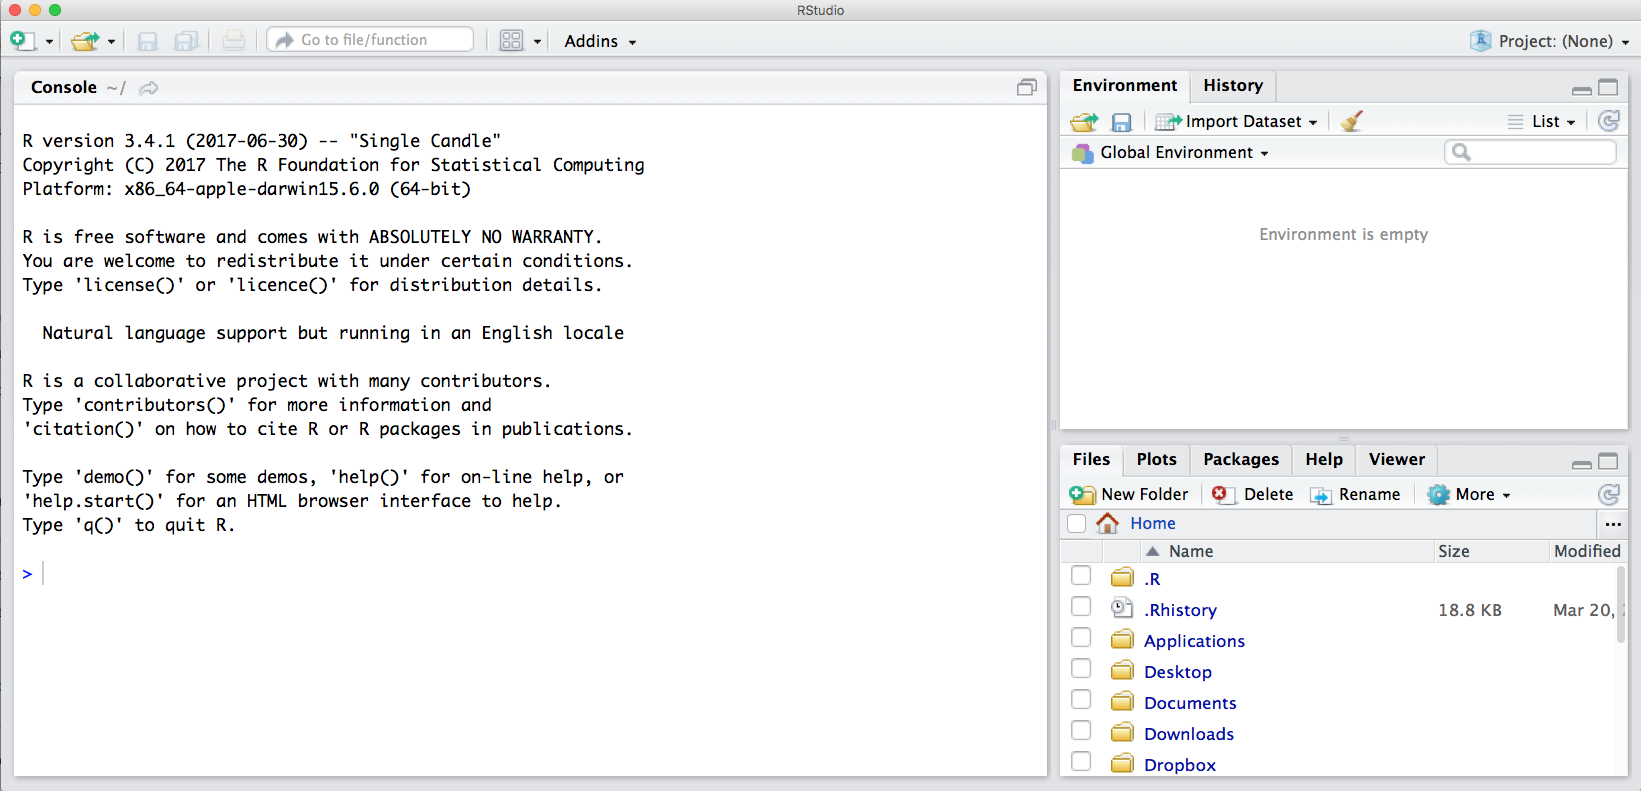
\includegraphics[width=0.8\linewidth]{img/RStudio_IDE}

Notice the default panes:

\begin{itemize}
\tightlist
\item
  Console (entire left)
\item
  Environment/History (tabbed in upper right)
\item
  Files/Plots/Packages/Help (tabbed in lower right)
\end{itemize}

FYI: you can change the default location of the panes, among many other things: \href{https://support.rstudio.com/hc/en-us/articles/200549016-Customizing-RStudio}{Customizing RStudio}.

An important first question: \textbf{where are we?}

If you've have opened RStudio for the first time, you'll be in your Home directory. This is noted by the \texttt{\textasciitilde{}/} at the top of the console. You can see too that the Files pane in the lower right shows what is in the Home directory where you are. You can navigate around within that Files pane and explore, but note that you won't change where you are: even as you click through you'll still be Home: \texttt{\textasciitilde{}/}.

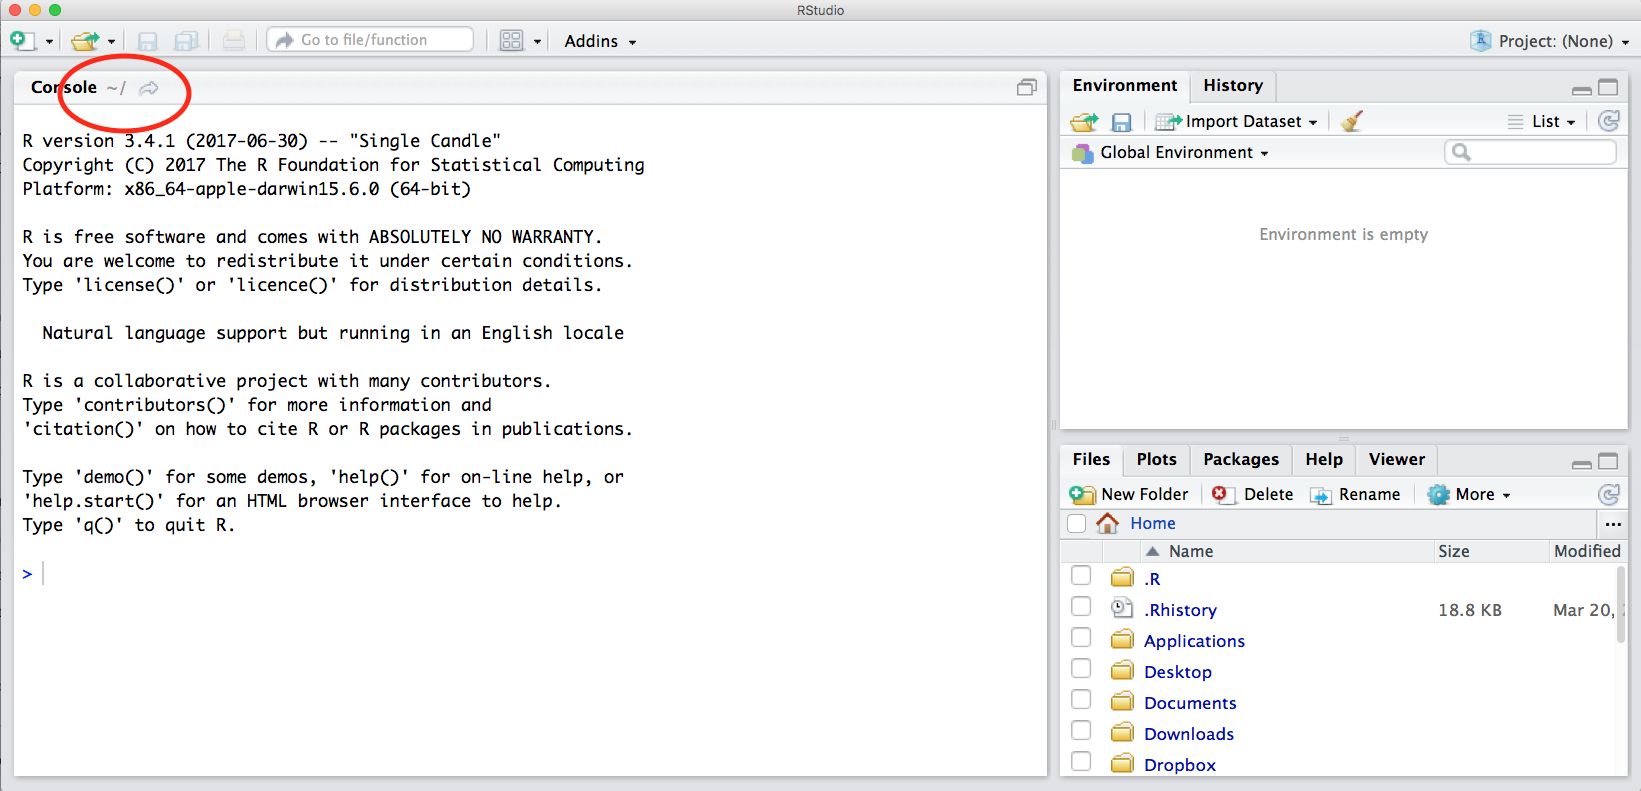
\includegraphics[width=0.8\linewidth]{img/RStudio_IDE_homedir}

\hypertarget{rstudio-projects}{%
\subsection{RStudio Projects}\label{rstudio-projects}}

Create a new Project called `r-for-excel-users'. File \textgreater{} New Project\ldots{} \textgreater{} New Directory \textgreater{} New Project. Give your Project a name browse to a place to keep it. And then click to Create Project!

What is a Project? It is a way to organize all of the relevant things you need for an analysis in the same place. This means data, code, figures, notes, etc.

Why does this matter? Keeping everything you need for your analysis together makes it less brittle and more portable --- across people, time, and computers.

Working directory = no file path/broken path issues. Notice that a folder now appears wherever you saved this project with the same name, and it contains a .Rproj file.

Now that we have our Project, here is an important question: where are we? Now we are in our Project. Everything we do will by default be saved here so we can be nice and organized.

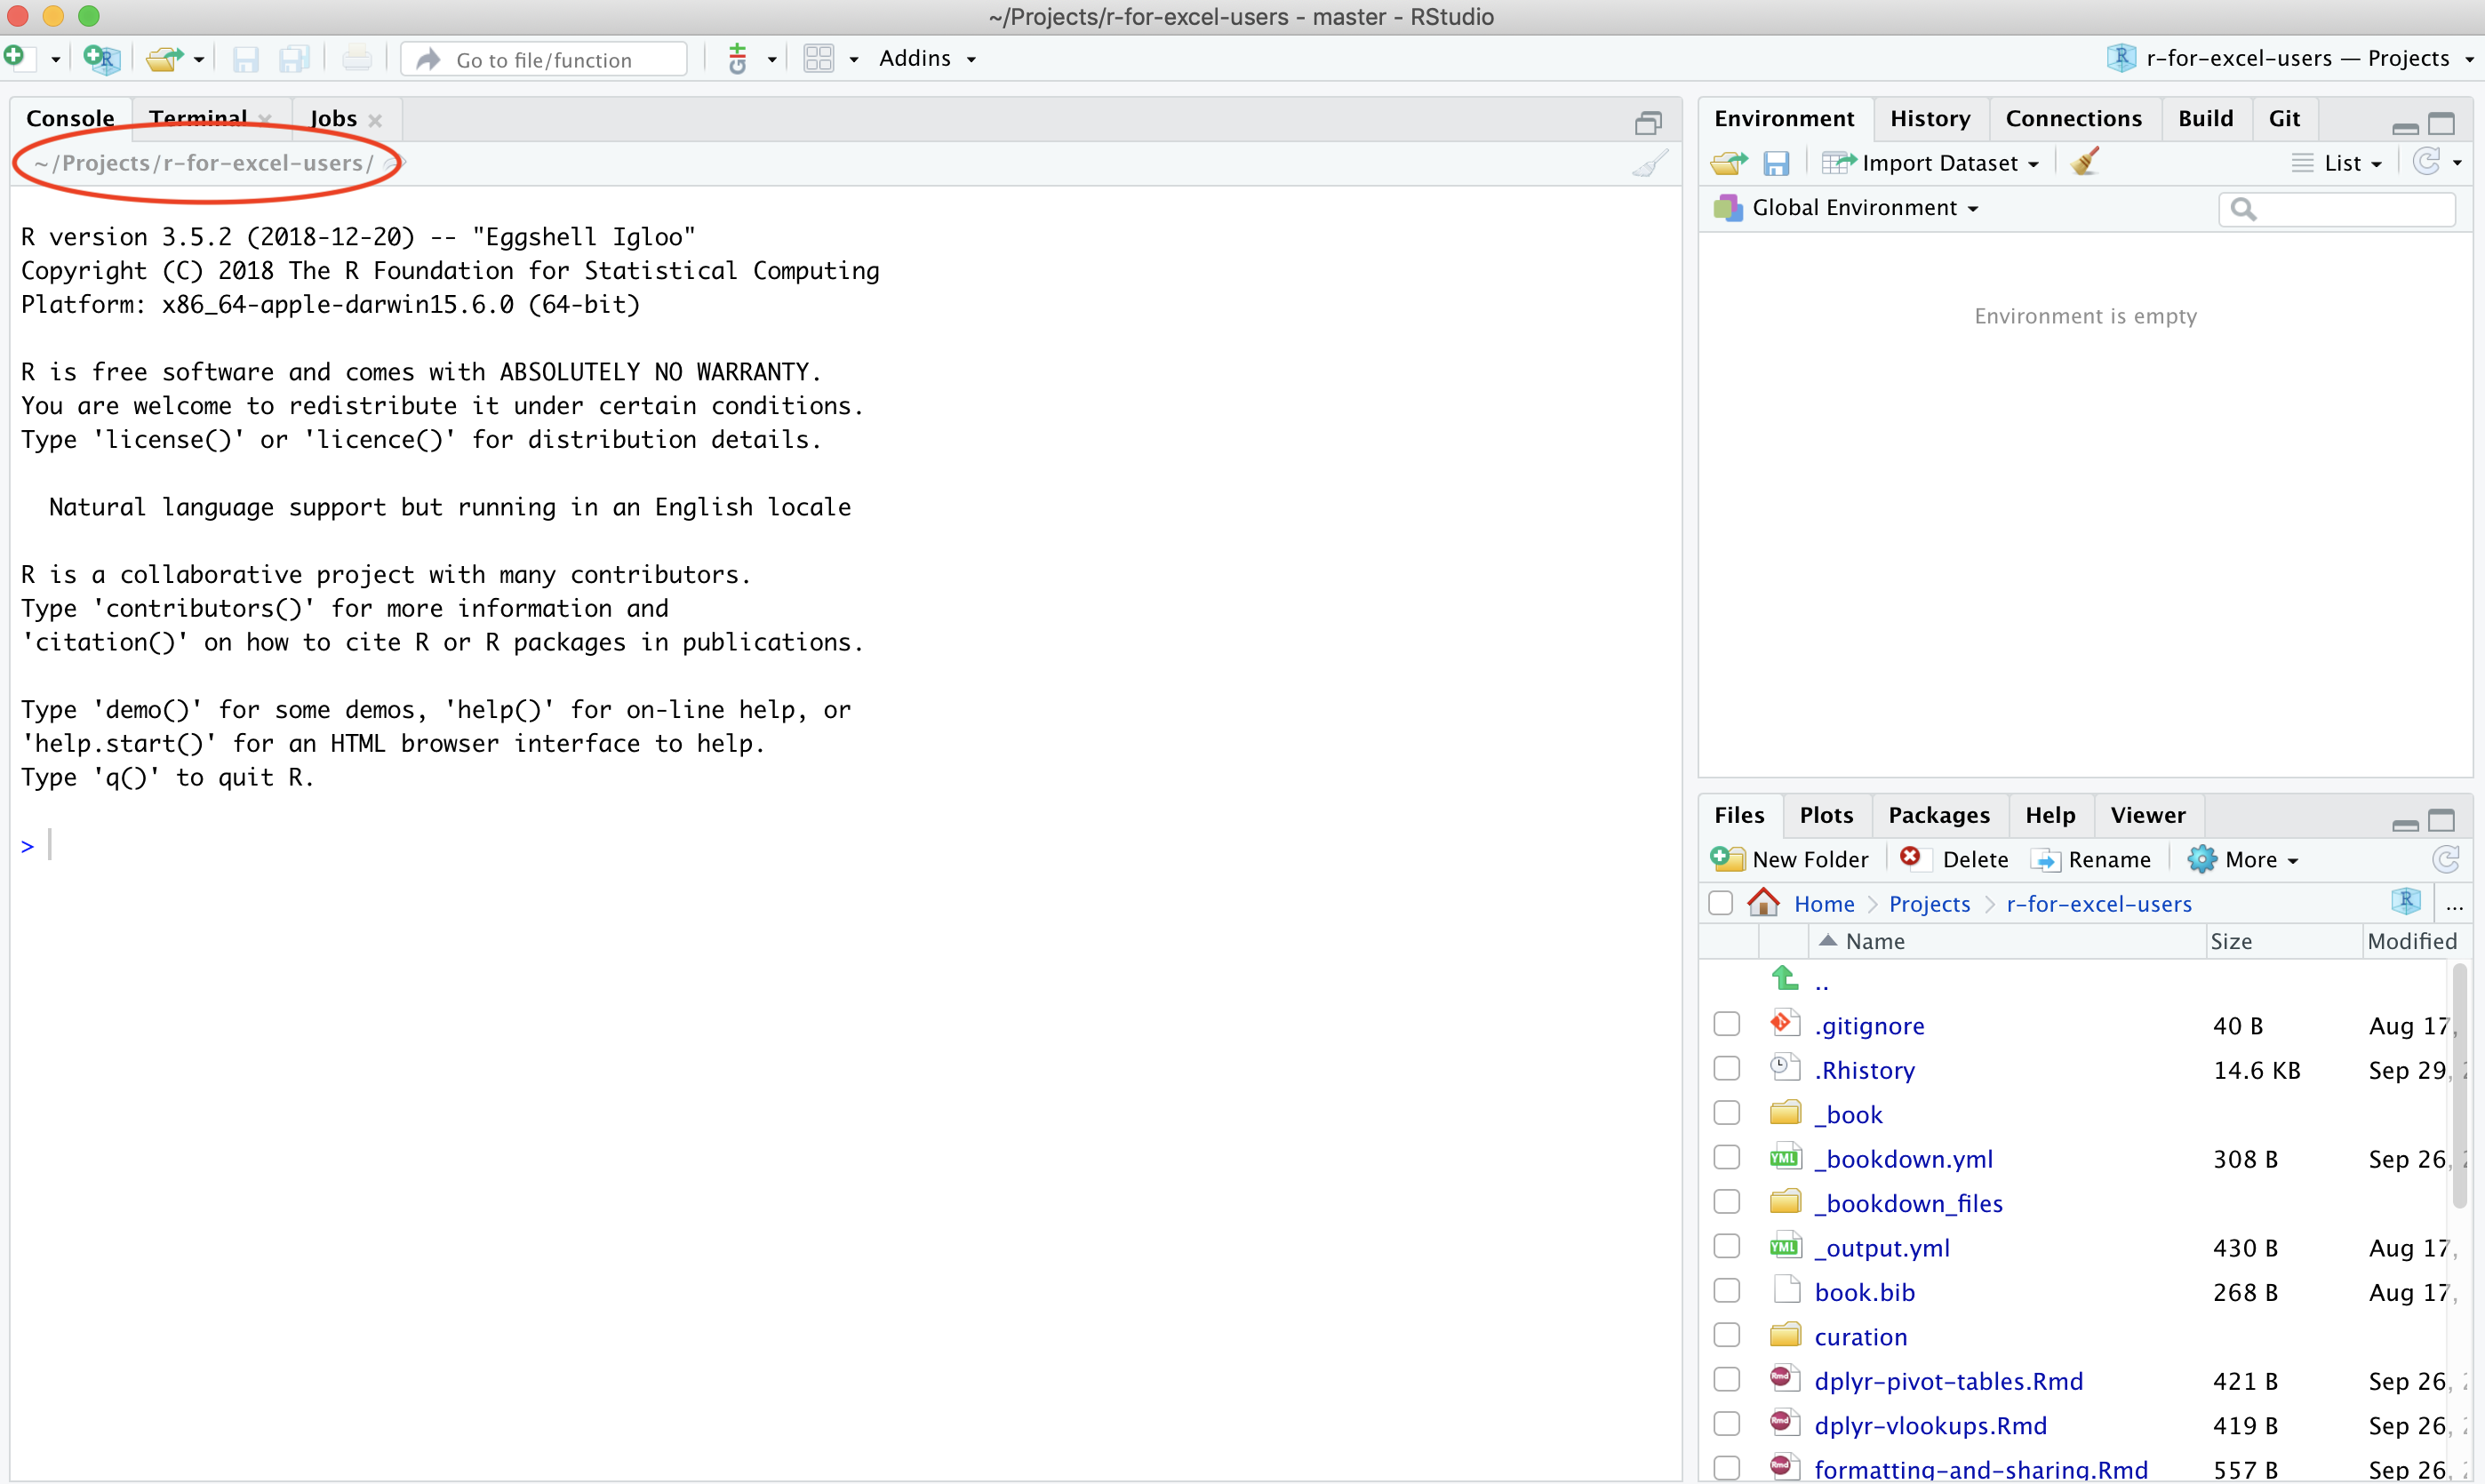
\includegraphics[width=0.8\linewidth]{img/RStudio_IDE_projdir}

\hypertarget{r-console}{%
\subsection{R Console}\label{r-console}}

Watch me work in the Console.

I can do math:

\begin{Shaded}
\begin{Highlighting}[]
\DecValTok{52}\OperatorTok{*}\DecValTok{40}
\DecValTok{365}\OperatorTok{/}\DecValTok{12}
\end{Highlighting}
\end{Shaded}

\emph{TODO: refine}

But like Excel, the power comes not from doing small operations by hand (like 8*22.3), it's by being able to operate on whole suites of numbers and datasets. In Excel, data are stored in the spreadsheet. In R, they are stored in dataframes, and named as variables.

R stores data in variables, and that data can be a variety of formats, like numeric and text.

Let's have a look at some data in R. R has several built-in data sets that we can look at and work with.

One of these datasets is called \texttt{mtcars}. If I write this in the Console, it will print the data in the console.

\begin{Shaded}
\begin{Highlighting}[]
\NormalTok{mtcars}
\end{Highlighting}
\end{Shaded}

I can also use RStudio's Viewer to see this in a more familiar-looking format:

\begin{Shaded}
\begin{Highlighting}[]
\KeywordTok{View}\NormalTok{(mtcars)}
\end{Highlighting}
\end{Shaded}

This opens the fourth pane of the RStudio IDE; when you work in R you will have all four panes open so this will become a very comforting setup for you.

In the Viewer I can do things like filter or sort. This does not do anything to the actual data, it just changes how you are viewing the data. So even as I explore it, I am not editing or manipulating the data.

Like Excel, some of the biggest power in R is that there are built-in functions that you can use in your analyses (and, as we'll see, R users can easily create and share functions, and it is this open source developer and contributor community that makes R so awesome).

So let's look into some of these functions. In Excel, there is a ``SUM'' function to calculate a total. Let's expect that there is the same in R. I will type this into the Console:

\begin{Shaded}
\begin{Highlighting}[]
\NormalTok{?sum}
\end{Highlighting}
\end{Shaded}

A few important things to note:

\begin{enumerate}
\def\labelenumi{\arabic{enumi}.}
\item
  R is case-sensitive. So ``sum'' is a completely different thing to ``Sum'' or ``SUM''. And this is true for the names of functions, data sets, variable names, and data itself (``blue'' vs ``Blue'').
\item
  RStudio has an autocomplete feature that can help you find the function you're looking for. In many cases it pops up as you type, but you can always type the tab key (above your caps lock key) to prompt the autocomplete. And, bonus: this feature can help you with the case-sensitivity mentioned above: If I start typing ``?SU'' and press tab, it will show me all options starting with those two letters, regardless of capitalization (although it will start with the capital S options).
\end{enumerate}

OK but what does typing \texttt{?sum} actually \emph{do}?

When I press enter/return, it will open up a help page in the bottom right pane. Help pages vary in detail I find some easier to digest than others. But they all have the same structure, which is helpful to know. The help page tells the name of the package in the top left, and broken down into sections:

\begin{itemize}
\tightlist
\item
  Description: An extended description of what the function does.
\item
  Usage: The arguments of the function and their default values.
\item
  Arguments: An explanation of the data each argument is expecting.
\item
  Details: Any important details to be aware of.
\item
  Value: The data the function returns.
\item
  See Also: Any related functions you might find useful.
\item
  Examples: Some examples for how to use the function.
\end{itemize}

When I look at a help page, I start with the description, which might be too in-the-weeds for the level of understanding I need at the offset. For the \texttt{sum} page, it is pretty straight-forward and lets me know that yup, this is the function I want.

I next look at the usage and arguments, which give me a more concrete view into what the function does. This syntax looks a bit cryptic but what it means is that you use it by writing sum, and then passing whatever you want to it in terms of data: that is what the ``\ldots{}'' means. And the ``na.rm=FALSE'' means that by default, it will not remove NAs (I read this as: ``remove NAs? FALSE!'')

Then, I usually scroll down to the bottom to the examples. This is where I can actually see how the function is used, and I can also paste those examples into the Console to see their output. Best way to learn what the function actually does is seeing it in action. Let's try:

\begin{Shaded}
\begin{Highlighting}[]
\KeywordTok{sum}\NormalTok{(}\DecValTok{1}\OperatorTok{:}\DecValTok{5}\NormalTok{)}
\end{Highlighting}
\end{Shaded}

So this is calculating the sum of the numbers from 1 and 5; that is what that \texttt{1:5} syntax means in this case. We can check it with the next example:

\begin{Shaded}
\begin{Highlighting}[]
\KeywordTok{sum}\NormalTok{(}\DecValTok{1}\NormalTok{, }\DecValTok{2}\NormalTok{, }\DecValTok{3}\NormalTok{, }\DecValTok{4}\NormalTok{, }\DecValTok{5}\NormalTok{)}
\end{Highlighting}
\end{Shaded}

Awesome. Let's try this on our \texttt{mtcars} data

\begin{Shaded}
\begin{Highlighting}[]
\KeywordTok{sum}\NormalTok{(mtcars)}
\end{Highlighting}
\end{Shaded}

Alright. What is this number? It is the sum of ALL of the data in the mtcars dataset. Maybe in some analysis this would be a useful operation, but I would worry about the way your data is set up and your analyses if this is ever something you'd want to do. More likely, you'd want to take the sum of a specific column. In R, you can do that with the \texttt{\$} operator.

Let's say we want to calculate the total number of gears that all these cars have:

\begin{Shaded}
\begin{Highlighting}[]
\KeywordTok{sum}\NormalTok{(mtcars}\OperatorTok{$}\NormalTok{gear)}
\end{Highlighting}
\end{Shaded}

OK so now that we've got a little bit of a feel for R and RStudio, let's do something much more interesting and really start feeling its power.

\hypertarget{r-scripts}{%
\section{R Scripts}\label{r-scripts}}

OK so working in the Console is great for quick things, but it gets messy. Keeping track at what I've done and trying to build upon it would be a nightmare.

Instead of working in the Console, we can be more organized by writing analyses in a script. This is a really powerful way to work in R. \emph{TODO dev more} Scripts are a written record of the analyses you do, unlike Excel. And they can be re-run easily\ldots{}

In this script, we're going to make our first figure in R. Let's all do this together.

File \textgreater{} New File \textgreater{} R Script.

This is a blank slate for us to write our code; but there are some good practices we can start off with. Let's add a useful header to the top of it. For example, at a minimum:

\begin{Shaded}
\begin{Highlighting}[]
\CommentTok{# --------------------------------}
\CommentTok{# A descriptive title}
\CommentTok{# Your name}
\CommentTok{# Contact information}
\CommentTok{# Date}
\CommentTok{# --------------------------------}
\end{Highlighting}
\end{Shaded}

And then let's save it, naming it something like ``my\_first\_figure.R''. Let's get into good habits now with this filename: no spaces! Use underscores \texttt{\_} or dashes \texttt{-} or no space at all.

Since we're working in or Project, this script is now nicely saved in our Project. You can see our \texttt{.R} show up in our Files pane on the bottom right.

Let's attach a package. Since you've already installed tidyverse,

\begin{Shaded}
\begin{Highlighting}[]
\CommentTok{# Attach the tidyverse}
\KeywordTok{library}\NormalTok{(tidyverse)}
\end{Highlighting}
\end{Shaded}

What is the tidyverse? \emph{TODO}
- ggplot2

Let's look at one of the datasets that is built into the ggplot2 package. Type this into your R script:

\begin{Shaded}
\begin{Highlighting}[]
\KeywordTok{View}\NormalTok{(diamonds)}
\end{Highlighting}
\end{Shaded}

So this is not immediately executed like when we were typing in the Console. That's because an R script is really just a text file that doesn't do anything on its own; you need to tell R to execute it. You do that in a few ways (let's do each of them):

\begin{enumerate}
\def\labelenumi{\arabic{enumi}.}
\tightlist
\item
  copy-paste this line into the console.
\item
  click Run (with green arrow at the top-right of your script) to run the line where your cursor is or any highlighted selection
\item
  click Source (top right of your script) to run the whole script.
\end{enumerate}

Now let's plot it. Type this or copy-paste and then we'll discuss:

\begin{Shaded}
\begin{Highlighting}[]
\KeywordTok{ggplot}\NormalTok{(diamonds, }\KeywordTok{aes}\NormalTok{(}\DataTypeTok{x =}\NormalTok{ carat, }\DataTypeTok{y =}\NormalTok{ price)) }\OperatorTok{+}
\StringTok{  }\KeywordTok{geom_point}\NormalTok{()}
\end{Highlighting}
\end{Shaded}

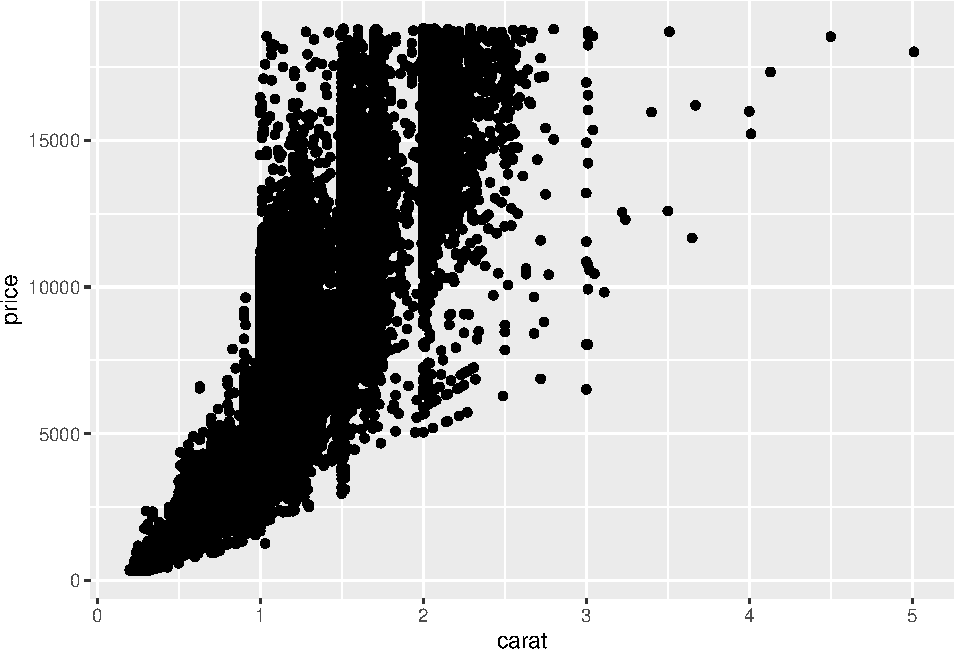
\includegraphics{R-for-Excel-Users_files/figure-latex/unnamed-chunk-8-1.pdf}

\hypertarget{deep-thought-error-messages-are-your-friends}{%
\subsection{Deep thought: Error messages are your friends}\label{deep-thought-error-messages-are-your-friends}}

Implicit contract with the computer / scripting language: Computer will do tedious computation for you. In return, you will be completely precise in your instructions. Typos matter. Case matters. Pay attention to how you type.

Remember that this is a language, not unsimilar to English! There are times you aren't understood -- it's going to happen. There are different ways this can happen. Sometimes you'll get an error. This is like someone saying `What?' or `Pardon'? Error messages can also be more useful, like when they say `I didn't understand what you said, I was expecting you to say blah'. That is a great type of error message. Error messages are your friend. Google them (copy-and-paste!) to figure out what they mean.

And also know that there are errors that can creep in more subtly, when you are giving information that is understood, but not in the way you meant. Like if I am telling a story about suspenders that my British friend hears but silently interprets in a very different way (true story). This can leave me thinking I've gotten something across that the listener (or R) might silently interpreted very differently. And as I continue telling my story you get more and more confused\ldots{} Clear communication is critical when you code: write clean, well documented code and check your work as you go to minimize these circumstances!

\hypertarget{the-pipe}{%
\section{The pipe \%\textgreater{}\%}\label{the-pipe}}

\hypertarget{dont-save-the-workspace}{%
\section{Don't save the workspace}\label{dont-save-the-workspace}}

\hypertarget{deep-thought-keep-the-raw-data-raw.}{%
\section{Deep thought: keep the raw data raw.}\label{deep-thought-keep-the-raw-data-raw.}}

Discussing using Excel for variables.

Horror Stories! Economist etc.

\hypertarget{interludes-deep-thoughtsopenscapes}{%
\section{Interludes (deep thoughts/openscapes)}\label{interludes-deep-thoughtsopenscapes}}

Comments! Organization (spacing, subsections, vertical structure, indentation, etc.)! Well-named variables! Also, well-named operations so analyses (select(data, columnname)) instead of data{[}1:6,5{]} and excel equivalent. (Ex with strings)
Not so brittle/sensitive to minor changes.

\hypertarget{activity-1}{%
\section{Activity 1}\label{activity-1}}

\hypertarget{activity-2}{%
\section{Activity 2}\label{activity-2}}

\hypertarget{efficiency-tips}{%
\section{Efficiency Tips}\label{efficiency-tips}}

\hypertarget{readxl}{%
\chapter{\texorpdfstring{\texttt{readxl}}{readxl}}\label{readxl}}

\hypertarget{summary}{%
\section{Summary}\label{summary}}

\textbf{Check this, may need to be a block quote}: The \textbf{readxl} package makes it easy to import tabular data from Excel spreadsheets (.xls or .xlsx files) and includes several options for cleaning data during import. \textbf{readxl} has no external dependencies and functions on any operating system, making it an OS- and user-friendly package that simplifies getting your data from Excel into R.

\hypertarget{objectives}{%
\section{Objectives}\label{objectives}}

\begin{itemize}
\tightlist
\item
  Use \texttt{readr::read\_csv()} to read in a comma separated value (CSV) file
\item
  Use \texttt{readxl::read\_excel()} to read in an Excel worksheet from a workbook
\item
  Replace a specific string/value in a spreadsheet with with \texttt{NA}
\item
  Skip \emph{n} rows when importing an Excel worksheet
\item
  Use \texttt{readxl::read\_excel()} to read in parts of a worksheet (by cell range)
\item
  Specify column names when importing Excel data
\item
  Read and combine data from multiple Excel worksheets into a single df using \texttt{purrr::map\_df()}
\item
  Write data using \texttt{readr::write\_csv()} or \texttt{writexl::write\_excel()}
\item
  Workflows with \texttt{readxl}: considerations, limitations, reproducibility
\end{itemize}

\hypertarget{resources-1}{%
\section{Resources}\label{resources-1}}

\begin{itemize}
\tightlist
\item
  \url{https://readxl.tidyverse.org/}
\item
  \href{https://readxl.tidyverse.org/articles/articles/readxl-workflows.html}{readxl Workflows article (from tidyverse.org)}
\end{itemize}

\hypertarget{lesson}{%
\section{Lesson}\label{lesson}}

\hypertarget{lesson-prep-get-data-files-into-your-working-directory}{%
\subsection{Lesson prep: get data files into your working directory}\label{lesson-prep-get-data-files-into-your-working-directory}}

In Session 1, we introduced how and why R Projects are great for reproducibility, because our self-contained working directory will be the \textbf{first} place R looks for files.

You downloaded four files for this workshop:

\begin{itemize}
\tightlist
\item
  fish\_counts\_curated.csv
\item
  invert\_counts\_curated.xlsx
\item
  kelp\_counts\_curated.xlsx
\item
  substrate\_cover\_curated.xlsx
\end{itemize}

Copy and paste those files into the `r-and-excel' folder on your computer. Notice that now these files are in your working directory when you go back to that Project in RStudio (check the `Files' tab). That means they're going to be in the first place R will look when you ask it to find a file to read in.

\hypertarget{create-a-new-.r-script-attach-the-tidyverse-readxl-and-writexl-packages}{%
\subsection{\texorpdfstring{Create a new .R script, attach the \texttt{tidyverse}, \texttt{readxl} and \texttt{writexl} packages}{Create a new .R script, attach the tidyverse, readxl and writexl packages}}\label{create-a-new-.r-script-attach-the-tidyverse-readxl-and-writexl-packages}}

In your RforExcelUsers project in RStudio, open a new .R script and add a useful header to the top of it. For example, at a minimum:

\begin{Shaded}
\begin{Highlighting}[]
\CommentTok{# --------------------------------}
\CommentTok{# A descriptive title}
\CommentTok{# Summary of what this script is for }
\CommentTok{# Your name}
\CommentTok{# Contact information}
\CommentTok{# --------------------------------}

\CommentTok{# Other things you might include: required packages or datasets, relevant links (e.g. to raw data source, GitHub repo, etc.), citations and sources.}
\end{Highlighting}
\end{Shaded}

In this lesson, we'll read in a CSV file with the \texttt{readr::read\_csv()} function, so we need to have the \texttt{readr} package attached. Since it's part of the \texttt{tidyverse}, we'll go ahead and attach the \texttt{tidyverse} package below our script header using \texttt{library(package\_name)}. It's a good idea to attach all necessary packages near the top of a script, so we'll also attach the \texttt{readxl} packages here.

\begin{Shaded}
\begin{Highlighting}[]
\CommentTok{# Attach the tidyverse, readxl and writexl packages:}
\KeywordTok{library}\NormalTok{(tidyverse)}
\KeywordTok{library}\NormalTok{(readxl)}
\KeywordTok{library}\NormalTok{(writexl)}
\end{Highlighting}
\end{Shaded}

Now, all of the packages and functions within the \texttt{tidyverse} and \texttt{readxl}, including \texttt{readr::read\_csv()} and \texttt{readxl::read\_excel()}, are available for use.

\hypertarget{use-readrread_csv-to-read-in-data-from-a-csv-file}{%
\subsection{\texorpdfstring{Use \texttt{readr::read\_csv()} to read in data from a CSV file}{Use readr::read\_csv() to read in data from a CSV file}}\label{use-readrread_csv-to-read-in-data-from-a-csv-file}}

There are many types of files containing data that you might want to work with in R. A common one is a comma separated value (CSV) file, which contains values with each column entry separated by a comma delimiter. CSVs can be opened, viewed, and worked with in Excel just like an .xls or .xlsx file - but let's learn how to get data directly from a CSV into R where we can work with it more reproducibly.

The CSV we'll read in here is called ``fish\_counts\_curated.csv'', and contains observations for ``the abundance and size of fish species as part of SBCLTER's kelp forest monitoring program to track long-term patterns in species abundance and diversity'' from the \href{http://sbc.lternet.edu/}{Santa Barbara Channel Long Term Ecological Research} program.

\textbf{Source:} Reed D. 2018. SBC LTER: Reef: Kelp Forest Community Dynamics: Fish abundance. Environmental Data Initiative. \url{https://doi.org/10.6073/pasta/dbd1d5f0b225d903371ce89b09ee7379}. Dataset accessed 9/26/2019.

Read in the ``fish\_counts\_curated.csv'' file \texttt{read\_csv("file\_name.csv")}, and store it in R as an object called \emph{fish\_counts}:

\begin{Shaded}
\begin{Highlighting}[]
\NormalTok{fish_counts <-}\StringTok{ }\KeywordTok{read_csv}\NormalTok{(}\StringTok{"fish_counts_curated.csv"}\NormalTok{)}
\end{Highlighting}
\end{Shaded}

Notice that the name of the stored object (here, \emph{fish\_counts}) will show up in our Environment tab in RStudio.

Click on the object in the Environment, and R will automatically run the \texttt{View()} function for you to pull up your data in a separate viewing tab. Now we can look at it in the spreadsheet format we're used to.

Here are a few other functions for quickly exploring imported data:

\begin{itemize}
\tightlist
\item
  \texttt{summary()}: summary of class, dimensions, \texttt{NA} values, etc.
\item
  \texttt{names()}: variable names (column headers)
\item
  \texttt{ls()}: list all objects in environment
\item
  \texttt{head()}: Show the first x rows (default is 6 lines)
\item
  \texttt{tail()}: Show the last x rows (default is 6 lines)
\end{itemize}

Now let's make a simple plot of some fish counts with \texttt{ggplot2}.

\begin{Shaded}
\begin{Highlighting}[]
\KeywordTok{ggplot}\NormalTok{(fish_counts, }\KeywordTok{aes}\NormalTok{(}\DataTypeTok{x =}\NormalTok{ year, }\DataTypeTok{y =}\NormalTok{ tot_count)) }\OperatorTok{+}
\StringTok{  }\KeywordTok{geom_col}\NormalTok{(}\KeywordTok{aes}\NormalTok{(}\DataTypeTok{fill =}\NormalTok{ common_name)) }\OperatorTok{+}
\StringTok{  }\KeywordTok{facet_wrap}\NormalTok{(}\OperatorTok{~}\NormalTok{site)}
\end{Highlighting}
\end{Shaded}

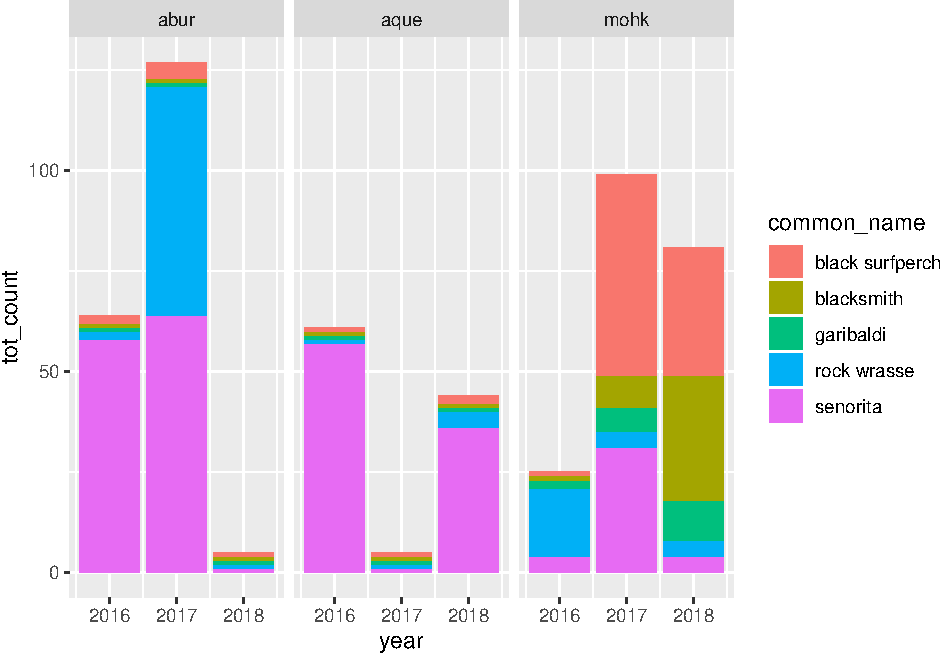
\includegraphics{R-for-Excel-Users_files/figure-latex/unnamed-chunk-13-1.pdf}

Now that we have our fish counts data ready to work with in R, let's get the substrate cover and kelp data (both .xlsx files). In the following sections, we'll learn that we can use \texttt{readxl::read\_excel()} to read in Excel files directly.

\hypertarget{use-readxlread_excel-to-read-in-a-single-excel-worksheet}{%
\subsection{\texorpdfstring{Use \texttt{readxl::read\_excel()} to read in a single Excel worksheet}{Use readxl::read\_excel() to read in a single Excel worksheet}}\label{use-readxlread_excel-to-read-in-a-single-excel-worksheet}}

First, take a look at \emph{substrate\_cover\_curated.xlsx} in Excel, which contains a single worksheet with substrate type and percent cover observations at different sampling locations in the Santa Barbara Channel.

A few things to notice:

\begin{itemize}
\tightlist
\item
  The file contains a single worksheet
\item
  There are multiple rows containing text information up top
\item
  Where observations were not recorded, there exists `-9999'
\end{itemize}

Let's go ahead and read in the data. If the file is in our working directory, we can read in a single worksheet .xlsx file using \texttt{readxl::read\_excel("file\_name.xlsx")}. \emph{Note: readxl::read\_excel() works for both .xlsx and .xls types}.

Like this:

\begin{Shaded}
\begin{Highlighting}[]
\NormalTok{substrate_cover <-}\StringTok{ }\KeywordTok{read_excel}\NormalTok{(}\StringTok{"substrate_cover_curated.xlsx"}\NormalTok{)}
\end{Highlighting}
\end{Shaded}

\textbf{Tada? Not quite.}

Click on the object name (\emph{substrate\_cover}) in the Environment to view the data in a new tab. A few things aren't ideal:

\begin{Shaded}
\begin{Highlighting}[]
\NormalTok{substrate_cover}
\end{Highlighting}
\end{Shaded}

\begin{verbatim}
## # A tibble: 23,942 x 9
##    `Substrate cover data~ ...2  ...3   ...4  ...5   ...6  ...7  ...8  ...9 
##    <chr>                  <chr> <chr>  <chr> <chr>  <chr> <chr> <chr> <chr>
##  1 Source: https://porta~ <NA>  <NA>   <NA>  <NA>   <NA>  <NA>  <NA>  <NA> 
##  2 Accessed: 9/28/2019    <NA>  <NA>   <NA>  <NA>   <NA>  <NA>  <NA>  <NA> 
##  3 <NA>                   <NA>  <NA>   <NA>  <NA>   <NA>  <NA>  <NA>  <NA> 
##  4 year                   month date   site  trans~ quad  side  subs~ perc~
##  5 -9999                  -9999 -9999  carp  1      20    i     b     -9999
##  6 2000                   9     -9999  carp  1      20    o     b     -9999
##  7 2000                   9     9/8/00 carp  1      20    i     b     100  
##  8 2000                   9     9/8/00 carp  1      20    o     b     100  
##  9 2000                   9     9/8/00 carp  1      40    i     b     100  
## 10 2000                   9     9/8/00 carp  1      40    o     b     100  
## # ... with 23,932 more rows
\end{verbatim}

\begin{itemize}
\tightlist
\item
  The top row of text has automatically become the (messy) column headers
\item
  There are multiple descriptive rows before we actually get to the data
\item
  There are -9999s that we want R to understand \texttt{NA} instead
\end{itemize}

We can deal with those issues by adding arguments within \texttt{read\_excel()}. Include argument \texttt{skip\ =\ n} to skip the first `n' rows when importing data, and \texttt{na\ =\ "this"} to replace ``this'' with \texttt{NA} when importing:

\begin{Shaded}
\begin{Highlighting}[]
\NormalTok{substrate_cover <-}\StringTok{ }\KeywordTok{read_excel}\NormalTok{(}\StringTok{"curation/substrate_cover_curated.xlsx, skip = 4, na = "}\OperatorTok{-}\DecValTok{9999}\StringTok{")}
\end{Highlighting}
\end{Shaded}

\begin{Shaded}
\begin{Highlighting}[]
\NormalTok{substrate_cover}
\end{Highlighting}
\end{Shaded}

\begin{verbatim}
## # A tibble: 23,938 x 9
##    year  month date  site  transect quad  side  substrate_type
##    <chr> <chr> <chr> <chr> <chr>    <chr> <chr> <chr>         
##  1 <NA>  <NA>  <NA>  carp  1        20    i     b             
##  2 2000  9     <NA>  carp  1        20    o     b             
##  3 2000  9     9/8/~ carp  1        20    i     b             
##  4 2000  9     9/8/~ carp  1        20    o     b             
##  5 2000  9     9/8/~ carp  1        40    i     b             
##  6 2000  9     9/8/~ carp  1        40    o     b             
##  7 2000  9     9/8/~ carp  2        20    i     b             
##  8 2000  9     9/8/~ carp  2        20    o     b             
##  9 2000  9     9/8/~ carp  2        40    i     b             
## 10 2000  9     9/8/~ carp  2        40    o     b             
## # ... with 23,928 more rows, and 1 more variable: percent_cover <chr>
\end{verbatim}

Check out \emph{substrate\_cover}, and see that the first row \emph{after} the 4 skipped are the column names, and all -9999s have been updated to \texttt{NA}. Hooray!

\hypertarget{use-readxlread_excel-to-read-in-only-part-of-an-excel-worksheet}{%
\subsection{\texorpdfstring{Use \texttt{readxl::read\_excel()} to read in only \emph{part} of an Excel worksheet}{Use readxl::read\_excel() to read in only part of an Excel worksheet}}\label{use-readxlread_excel-to-read-in-only-part-of-an-excel-worksheet}}

We always advocate for leaving the raw data raw, and writing a complete script containing all steps of data wrangling \& transformation. But in \emph{some} situations (be careful), you may want to specify a range of cells to read in from an Excel worksheet.

You can specify a range of cells to read in using the \texttt{range\ =} argument in \texttt{read\_excel()}. For example, if I want to read in the rectangle from D12:I15 in \emph{substrate\_cover\_curated.xlsx} - only observations for Carpenteria Beach (Transect 2) in September 2000 - I can use:

\begin{Shaded}
\begin{Highlighting}[]
\NormalTok{carp_cover_}\DecValTok{2000}\NormalTok{ <-}\StringTok{ }\NormalTok{readxl}\OperatorTok{::}\KeywordTok{read_excel}\NormalTok{(}\StringTok{"substrate_cover_curated.xlsx"}\NormalTok{, }\DataTypeTok{range =} \StringTok{"D12:I15"}\NormalTok{)}
\end{Highlighting}
\end{Shaded}

But yuck. Look at \emph{carp\_cover\_2000} and you'll notice that the first row \emph{of that range} is automatically made the column headers. To keep all rows within a range and \textbf{add your own column names}, add a \texttt{col\_names\ =} argument:

\begin{Shaded}
\begin{Highlighting}[]
\NormalTok{carp_cover_}\DecValTok{2000}\NormalTok{ <-}\StringTok{ }\NormalTok{readxl}\OperatorTok{::}\KeywordTok{read_excel}\NormalTok{(}\StringTok{"substrate_cover_curated.xlsx"}\NormalTok{, }\DataTypeTok{range =} \StringTok{"D12:I15"}\NormalTok{, }\DataTypeTok{col_names =} \KeywordTok{c}\NormalTok{(}\StringTok{"site_name"}\NormalTok{, }\StringTok{"transect"}\NormalTok{, }\StringTok{"quad"}\NormalTok{, }\StringTok{"plot_side"}\NormalTok{, }\StringTok{"type"}\NormalTok{, }\StringTok{"coverage"}\NormalTok{))}
\end{Highlighting}
\end{Shaded}

\begin{Shaded}
\begin{Highlighting}[]
\NormalTok{carp_cover_}\DecValTok{2000}
\end{Highlighting}
\end{Shaded}

\begin{verbatim}
## # A tibble: 4 x 6
##   site_name transect quad  plot_side type  coverage
##   <chr>     <chr>    <chr> <chr>     <chr> <chr>   
## 1 carp      2        20    i         b     90      
## 2 carp      2        20    o         b     80      
## 3 carp      2        40    i         b     80      
## 4 carp      2        40    o         b     85
\end{verbatim}

So far we've read in a single CSV file using \texttt{readr::read\_csv()}, and an Excel file containing a single worksheet with \texttt{readxl::read\_excel()}. Now let's read in data from an Excel workbook with multiple worksheets.

\hypertarget{use-readxlread_excel-to-read-in-selected-worksheets-from-a-workbook}{%
\subsection{\texorpdfstring{Use \texttt{readxl::read\_excel()} to read in selected worksheets from a workbook}{Use readxl::read\_excel() to read in selected worksheets from a workbook}}\label{use-readxlread_excel-to-read-in-selected-worksheets-from-a-workbook}}

Now, we'll read in the kelp fronds data from file \emph{kelp\_counts\_curated.xlsx}. If you open the Excel workbook, you'll see that it contains multiple worksheets with giant kelp observations in the Santa Barbara Channel during July 2016, 2017, and 2018, with data collected at each \emph{site} in a separate worksheet.

To read in a single Excel worksheet from a workbook we'll again use \texttt{readxl::read\_excel("file\_name.xlsx")}, but we'll need to let R know which worksheet to get.

Let's read in the kelp data just like we did above, as an object called \emph{kelp\_counts}.

\begin{Shaded}
\begin{Highlighting}[]
\NormalTok{kelp_counts <-}\StringTok{ }\NormalTok{readxl}\OperatorTok{::}\KeywordTok{read_excel}\NormalTok{(}\StringTok{"kelp_counts_curated.xlsx"}\NormalTok{)}
\end{Highlighting}
\end{Shaded}

You might be thinking, ``Hooray, I got all of my Excel workbook data!'' But remember to always look at your data - you will see that actually only the first worksheet was read in. The default in \texttt{readxl::read\_excel()} is to read in the \textbf{first worksheet} in a multi-sheet Excel workbook.

To check the worksheet names in an Excel workbook, use \texttt{readxl::excel\_sheets()}:

\begin{Shaded}
\begin{Highlighting}[]
\NormalTok{readxl}\OperatorTok{::}\KeywordTok{excel_sheets}\NormalTok{(}\StringTok{"kelp_counts_curated.xlsx"}\NormalTok{)}
\end{Highlighting}
\end{Shaded}

If we want to read in data from a worksheet other than the first one in an Excel workbook, we can specify the correct worksheet by name or position by adding the \texttt{sheet} argument.

Let's read in data from the worksheet named \emph{golb} (Goleta Beach) in the \emph{kelp\_counts\_curated.xlsx} workbook:

\begin{Shaded}
\begin{Highlighting}[]
\NormalTok{kelp_golb <-}\StringTok{ }\NormalTok{readxl}\OperatorTok{::}\KeywordTok{read_excel}\NormalTok{(}\StringTok{"kelp_counts_curated.xlsx"}\NormalTok{, }\DataTypeTok{sheet =} \StringTok{"golb"}\NormalTok{)}
\end{Highlighting}
\end{Shaded}

Note that you can also specify a worksheet by position: since \emph{golb} is the 6\textsuperscript{th} worksheet in the workbook, we could also use the following:

\begin{Shaded}
\begin{Highlighting}[]
\NormalTok{kelp_golb <-}\StringTok{ }\NormalTok{readxl}\OperatorTok{::}\KeywordTok{read_excel}\NormalTok{(}\StringTok{"kelp_counts_curated.xlsx"}\NormalTok{, }\DataTypeTok{sheet =} \DecValTok{6}\NormalTok{)}
\end{Highlighting}
\end{Shaded}

\begin{Shaded}
\begin{Highlighting}[]
\NormalTok{kelp_golb}
\end{Highlighting}
\end{Shaded}

\begin{verbatim}
## # A tibble: 3 x 5
##   year  month site  common_name tot_fronds
##   <chr> <chr> <chr> <chr>            <dbl>
## 1 2016  7     golb  giant kelp        2557
## 2 2017  7     golb  giant kelp        1575
## 3 2018  7     golb  giant kelp        1629
\end{verbatim}

\hypertarget{read-in-and-combine-data-from-multiple-worksheets-into-a-data-frame-simultaneously-with-purrrmap_df}{%
\subsection{\texorpdfstring{Read in and combine data from multiple worksheets into a data frame simultaneously with \texttt{purrr::map\_df()}}{Read in and combine data from multiple worksheets into a data frame simultaneously with purrr::map\_df()}}\label{read-in-and-combine-data-from-multiple-worksheets-into-a-data-frame-simultaneously-with-purrrmap_df}}

So far, we've read in entire Excel worksheets and pieces of a worksheet. What if we have a workbook (like \emph{kelp\_counts\_curated.xlsx}) that contains worksheets that contain observations for the same variables, in the same organization? Then we may want to read in data from \emph{all} worksheets, and combine them into a single data frame.

We'll use \texttt{purrr::map\_df()} to loop through all the worksheets in a workbook, reading them in \& putting them together into a single df in the process.

The steps we'll go through in the code below are:

\begin{itemize}
\tightlist
\item
  Set a pathway so that R knows where to look for an Excel workbook
\item
  Get the names of all worksheets in that workbook with \texttt{excel\_sheets()}
\item
  Set names of a vector with \texttt{set\_names()}
\item
  Read in all worksheets, and put them together into a single data frame with \texttt{purrr::map\_df()}
\end{itemize}

\textbf{QUESTION: Have they learned the pipe operator at this point?}

\textbf{Expect the question:} Why do I need to use read\_excel() instead of just giving it the file path (as below)?

\begin{Shaded}
\begin{Highlighting}[]
\NormalTok{kelp_path <-}\StringTok{ "kelp_counts_curated.xlsx"}

\NormalTok{kelp_all_sites <-}\StringTok{ }\NormalTok{kelp_path }\OperatorTok\StringTok{ }
\StringTok{  }\KeywordTok{excel_sheets}\NormalTok{() }\OperatorTok\StringTok{ }
\StringTok{  }\KeywordTok{set_names}\NormalTok{() }\OperatorTok\StringTok{ }
\StringTok{  }\NormalTok{purrr}\OperatorTok{::}\KeywordTok{map_df}\NormalTok{(read_excel, kelp_path)}
\end{Highlighting}
\end{Shaded}

Check out \emph{kelp\_all\_sites}, and notice that now the data from all 11 sites is now collected into a single data frame:

\begin{Shaded}
\begin{Highlighting}[]
\NormalTok{kelp_all_sites}
\end{Highlighting}
\end{Shaded}

\begin{verbatim}
## # A tibble: 32 x 5
##    year  month site  common_name tot_fronds
##    <chr> <chr> <chr> <chr>            <dbl>
##  1 2016  7     abur  giant kelp         307
##  2 2017  7     abur  giant kelp         604
##  3 2018  7     abur  giant kelp        3532
##  4 2016  7     ahnd  giant kelp        2572
##  5 2017  7     ahnd  giant kelp          16
##  6 2018  7     ahnd  giant kelp          16
##  7 2016  7     aque  giant kelp       11152
##  8 2017  7     aque  giant kelp        9194
##  9 2018  7     aque  giant kelp        7754
## 10 2016  7     bull  giant kelp        6706
## # ... with 22 more rows
\end{verbatim}

Awesome! Let's make a graph with ggplot2:

\begin{Shaded}
\begin{Highlighting}[]
\KeywordTok{ggplot}\NormalTok{(kelp_all_sites, }\KeywordTok{aes}\NormalTok{(}\DataTypeTok{x =}\NormalTok{ site, }\DataTypeTok{y =}\NormalTok{ tot_fronds)) }\OperatorTok{+}
\StringTok{  }\KeywordTok{geom_col}\NormalTok{(}\KeywordTok{aes}\NormalTok{(}\DataTypeTok{fill =}\NormalTok{ year), }\DataTypeTok{position =} \StringTok{"dodge"}\NormalTok{) }\OperatorTok{+}
\StringTok{  }\KeywordTok{scale_fill_manual}\NormalTok{(}\DataTypeTok{values =} \KeywordTok{c}\NormalTok{(}\StringTok{"purple"}\NormalTok{,}\StringTok{"orange"}\NormalTok{,}\StringTok{"gray30"}\NormalTok{))}
\end{Highlighting}
\end{Shaded}

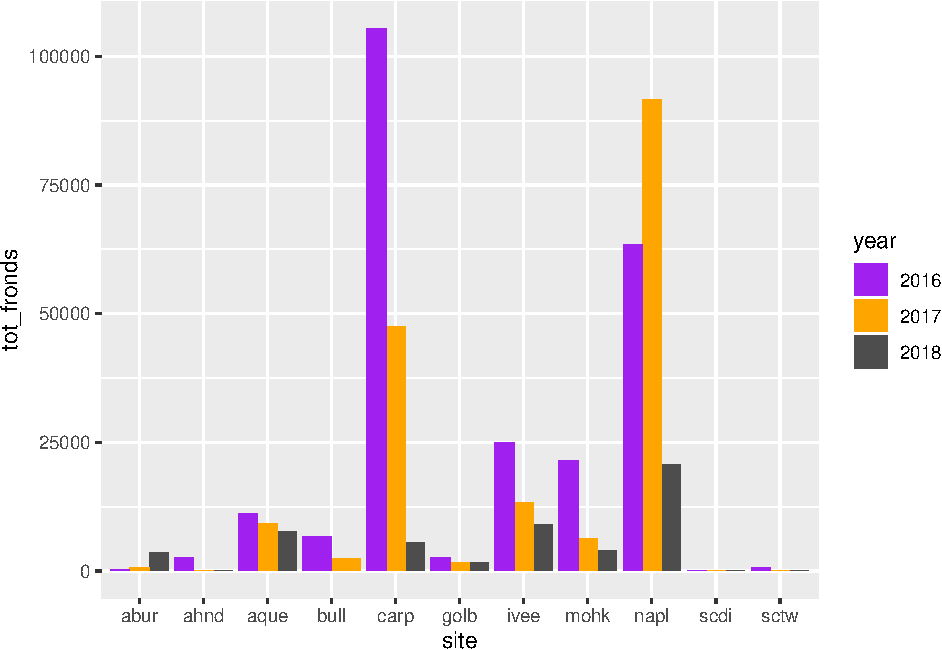
\includegraphics{R-for-Excel-Users_files/figure-latex/unnamed-chunk-37-1.pdf}

\hypertarget{save-data-frames-as-.csv-or-.xlsx-with-readrwrite_csv-or-writexlwrite_xlsx}{%
\subsection{\texorpdfstring{Save data frames as .csv or .xlsx with \texttt{readr::write\_csv()} or \texttt{writexl::write\_xlsx()}}{Save data frames as .csv or .xlsx with readr::write\_csv() or writexl::write\_xlsx()}}\label{save-data-frames-as-.csv-or-.xlsx-with-readrwrite_csv-or-writexlwrite_xlsx}}

There are a number of reasons you might want to save (/export) data in a data frame as a .csv or Excel worksheet, including:

\begin{itemize}
\tightlist
\item
  To cache raw data within your project
\item
  To store copies of intermediate data frames
\item
  To convert your data back to a format that your coworkers/clients/colleagues will be able to use it more easily
\end{itemize}

Use \texttt{readr::write\_csv(object,\ "file\_name.csv")} to write a data frame to a CSV, or \texttt{writexl::write\_xlsx(object,\ "file\_name.xlsx")} to similarly export as a .xlsx (or .xls) worksheet.

In the previous step, we combined all of our kelp frond observations into a single data frame. Wouldn't it make sense to store a copy?

As a CSV:

\begin{Shaded}
\begin{Highlighting}[]
\NormalTok{readr}\OperatorTok{::}\KeywordTok{write_csv}\NormalTok{(kelp_all_sites, }\StringTok{"kelp_all_sites.csv"}\NormalTok{)}
\end{Highlighting}
\end{Shaded}

A cool thing about \texttt{readr::read\_csv()} is that it just quietly \emph{works} without wrecking anything else you do in a sequence, so it's great to add at the end of a piped sequence.

For example, if I want to read in the `ivee' worksheet from kelp\_counts\_curated.xlsx, select only columns `year' and `tot\_fronds', then write that new subset to a .csv file, I can pipe all the way through:

\begin{Shaded}
\begin{Highlighting}[]
\NormalTok{kelp_ivee <-}\StringTok{ }\NormalTok{readxl}\OperatorTok{::}\KeywordTok{read_excel}\NormalTok{(}\StringTok{"kelp_counts_curated.xlsx"}\NormalTok{, }\DataTypeTok{sheet =} \StringTok{"ivee"}\NormalTok{) }\OperatorTok\StringTok{ }
\StringTok{  }\KeywordTok{select}\NormalTok{(year, tot_fronds) }\OperatorTok\StringTok{ }
\StringTok{  }\KeywordTok{write_csv}\NormalTok{(}\StringTok{"kelp_ivee.csv"}\NormalTok{)}
\end{Highlighting}
\end{Shaded}

Now I've created \emph{kelp\_ivee.csv}, but the object \emph{kelp\_ivee} also exists for me to use in R.

If needed, I can also export a data frame as an Excel (.xlsx) worksheet:

\begin{Shaded}
\begin{Highlighting}[]
\NormalTok{writexl}\OperatorTok{::}\KeywordTok{write_xlsx}\NormalTok{(kelp_all_sites, }\StringTok{"kelp_all_sites.xlsx"}\NormalTok{)}
\end{Highlighting}
\end{Shaded}

\hypertarget{fun-facts-ideas}{%
\section{Fun facts ideas:}\label{fun-facts-ideas}}

\begin{itemize}
\tightlist
\item
  Did you know that Clippy shows up to help you in the documentation for ?writexl::write\_xlsx()?
\item
  The name of the \texttt{purrr} package? Why map?
\end{itemize}

\hypertarget{interludes-deep-thoughtsopenscapes-1}{%
\section{Interludes (deep thoughts/openscapes)}\label{interludes-deep-thoughtsopenscapes-1}}

\begin{itemize}
\tightlist
\item
  Workflow/reproducibility/readxl workflows article
\item
  Respecting the tools people are working with already (e.g.~don't make your Excel using co-workers hate you)
\end{itemize}

\hypertarget{activity-import-some-invertebrates}{%
\section{Activity: Import some invertebrates!}\label{activity-import-some-invertebrates}}

There's one dataset we haven't imported or explored yet: invertebrate counts for 5 popular invertebrates (California cone snail, California spiny lobster, orange cup coral, purple urchin and rock scallops) at 11 sites in the Santa Barbara Channel. Take a look at the \emph{invert\_counts\_curated.xlsx} data by opening it in Excel

\begin{itemize}
\tightlist
\item
  Read in the \emph{invert\_counts\_curated.xlsx} worksheet as object `inverts\_july', only retaining \textbf{site}, \textbf{common\_name}, and \textbf{2016} and setting the existing first row in the worksheet as to column headers upon import
\item
  Explore the imported data frame using View, names, head, tail, etc.
\item
  Write `inverts\_july' to a CSV file in your working directory called ``inverts\_july.csv''
\item
  Create a basic graph of invert counts in 2016 (y-axis) by site (x-axis), with each species indicated by a different fill color

  \begin{itemize}
  \tightlist
  \item
    \textbf{Note:} If your column name is a number (not great) you'll probably want to rename it\ldots{}but in the meantime, to call it as a variable make sure you put single or double quotes around it (e.g. \texttt{\textquotesingle{}2016\textquotesingle{}} or \texttt{"2016"}) so that R recognizes it's a variable and not a value
  \end{itemize}
\end{itemize}

\begin{Shaded}
\begin{Highlighting}[]
\CommentTok{# Importing only 'site' through '2016' columns: }
\NormalTok{inverts_july <-}\StringTok{ }\NormalTok{readxl}\OperatorTok{::}\KeywordTok{read_excel}\NormalTok{(}\StringTok{"curation/invert_counts_curated.xlsx"}\NormalTok{, }\DataTypeTok{range =} \StringTok{"B1:D56"}\NormalTok{)}

\CommentTok{# Do some basic exploring (why might we want to do this in the Console instead?):}
\CommentTok{#View(inverts_july)}
\KeywordTok{names}\NormalTok{(inverts_july)}
\KeywordTok{head}\NormalTok{(inverts_july)}
\KeywordTok{tail}\NormalTok{(inverts_july)}
\KeywordTok{ls}\NormalTok{()}

\CommentTok{# Make a gg-graph plot: }
\NormalTok{inverts_graph <-}\StringTok{ }\KeywordTok{ggplot}\NormalTok{(inverts_july, }\KeywordTok{aes}\NormalTok{(}\DataTypeTok{x =}\NormalTok{ site, }\DataTypeTok{y =} \StringTok{`}\DataTypeTok{2016}\StringTok{`}\NormalTok{)) }\OperatorTok{+}
\StringTok{  }\KeywordTok{geom_col}\NormalTok{(}\KeywordTok{aes}\NormalTok{(}\DataTypeTok{fill =}\NormalTok{ common_name), }
           \DataTypeTok{position =} \StringTok{"dodge"}\NormalTok{)}
\end{Highlighting}
\end{Shaded}

\begin{Shaded}
\begin{Highlighting}[]
\NormalTok{inverts_graph}
\end{Highlighting}
\end{Shaded}

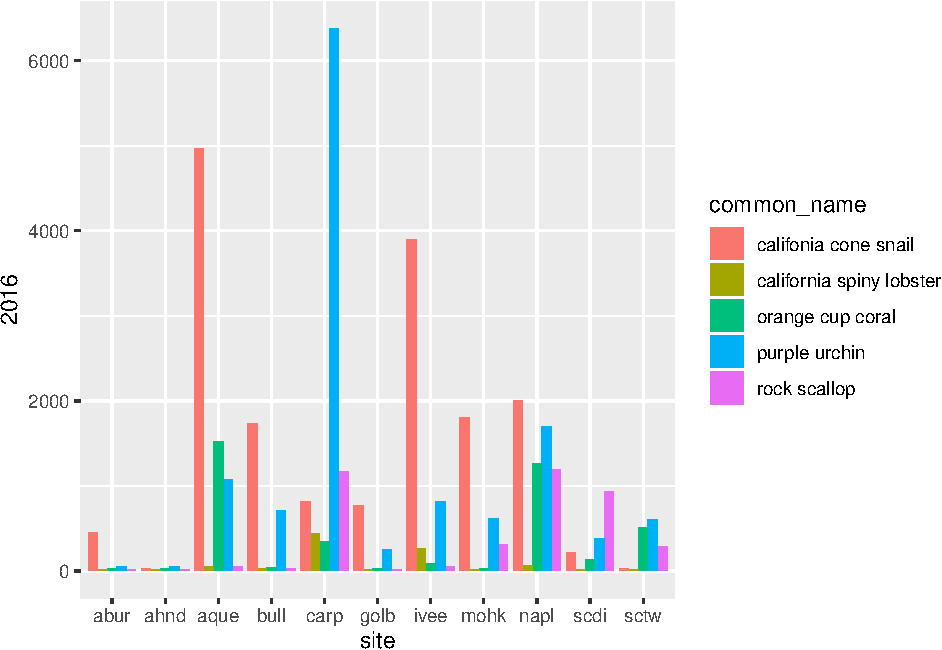
\includegraphics{R-for-Excel-Users_files/figure-latex/unnamed-chunk-44-1.pdf}

\hypertarget{efficiency-tips-1}{%
\section{Efficiency Tips}\label{efficiency-tips-1}}

\begin{itemize}
\tightlist
\item
  Add an assignment arrow in script/code chunk (\textless{}-): Alt + minus (-)
\item
  Undo shortcut: Command + Z
\item
  Redo shortcut: Command + Shift + Z
\end{itemize}

\hypertarget{rmarkdown}{%
\chapter{RMarkdown}\label{rmarkdown}}

\hypertarget{summary-a-few-sentences-1}{%
\section{Summary (a few sentences)}\label{summary-a-few-sentences-1}}

\hypertarget{objectives-more-detailed-bulletpoints-1}{%
\section{Objectives (more detailed, bulletpoints?)}\label{objectives-more-detailed-bulletpoints-1}}

\hypertarget{resources-2}{%
\section{Resources}\label{resources-2}}

\hypertarget{lessons-teaching-for-each-objective..-objectives-examples}{%
\section{Lessons teaching for each objective\ldots{}.. (objectives, examples)}\label{lessons-teaching-for-each-objective..-objectives-examples}}

Now, hitting return does not execute this command; remember, it's a text file in the text editor, it's not associated with the R engine. To execute it, we need to get what we typed in the the R chunk (the grey R code) down into the console. How do we do it? There are several ways (let's do each of them):

\begin{enumerate}
\def\labelenumi{\arabic{enumi}.}
\tightlist
\item
  copy-paste this line into the console.
\item
  select the line (or simply put the cursor there), and click `Run'. This is available from

  \begin{enumerate}
  \def\labelenumii{\alph{enumii}.}
  \tightlist
  \item
    the bar above the file (green arrow)
  \item
    the menu bar: Code \textgreater{} Run Selected Line(s)
  \item
    keyboard shortcut: command-return
  \end{enumerate}
\item
  click the green arrow at the right of the code chunk
\end{enumerate}

\hypertarget{fun-facts-quirky-things---making-a-note-of-these-wherever-possible-for-interest-little-did-you-know-sections}{%
\section{Fun facts (quirky things) - making a note of these wherever possible for interest (little ``Did you know?'' sections)}\label{fun-facts-quirky-things---making-a-note-of-these-wherever-possible-for-interest-little-did-you-know-sections}}

\hypertarget{interludes-deep-thoughtsopenscapes-2}{%
\section{Interludes (deep thoughts/openscapes)}\label{interludes-deep-thoughtsopenscapes-2}}

\hypertarget{our-turn-your-turn-1}{%
\section{Our Turn Your Turn 1}\label{our-turn-your-turn-1}}

\hypertarget{our-turn-your-turn-2}{%
\section{Our Turn Your Turn 2}\label{our-turn-your-turn-2}}

\hypertarget{efficiency-tips-2}{%
\section{Efficiency Tips}\label{efficiency-tips-2}}

\hypertarget{pivot}{%
\chapter{Dplyr and Pivot Tables}\label{pivot}}

\hypertarget{summary-a-few-sentences-2}{%
\section{Summary (a few sentences)}\label{summary-a-few-sentences-2}}

\hypertarget{objectives-more-detailed-bulletpoints-2}{%
\section{Objectives (more detailed, bulletpoints?)}\label{objectives-more-detailed-bulletpoints-2}}

\hypertarget{resources-3}{%
\section{Resources}\label{resources-3}}

\hypertarget{lessons-teaching-for-each-objective..-objectives-examples-1}{%
\section{Lessons teaching for each objective\ldots{}.. (objectives, examples)}\label{lessons-teaching-for-each-objective..-objectives-examples-1}}

\hypertarget{fun-facts-quirky-things---making-a-note-of-these-wherever-possible-for-interest-little-did-you-know-sections-1}{%
\section{Fun facts (quirky things) - making a note of these wherever possible for interest (little ``Did you know?'' sections)}\label{fun-facts-quirky-things---making-a-note-of-these-wherever-possible-for-interest-little-did-you-know-sections-1}}

\hypertarget{interludes-deep-thoughtsopenscapes-3}{%
\section{Interludes (deep thoughts/openscapes)}\label{interludes-deep-thoughtsopenscapes-3}}

\hypertarget{our-turn-your-turn-1-1}{%
\section{Our Turn Your Turn 1}\label{our-turn-your-turn-1-1}}

\hypertarget{our-turn-your-turn-2-1}{%
\section{Our Turn Your Turn 2}\label{our-turn-your-turn-2-1}}

\hypertarget{efficiency-tips-3}{%
\section{Efficiency Tips}\label{efficiency-tips-3}}

\hypertarget{vlookup}{%
\chapter{Dplyr and vlookups}\label{vlookup}}

\hypertarget{summary-a-few-sentences-3}{%
\section{Summary (a few sentences)}\label{summary-a-few-sentences-3}}

In Session 4, we learned how to do some basic wrangling and find summary information with functions in the \texttt{dplyr} package, which exists within the \texttt{tidyverse}. Those were:

TODO: Check this list (to see what actually gets covered in Session 4)

\begin{itemize}
\tightlist
\item
  \texttt{dplyr::select()}: select which \textbf{columns} to retain or exclude
\item
  \texttt{dplyr::mutate()}: \textbf{add} a new column, while keeping the existing ones
\item
  \texttt{dplyr::group\_by()}: let R know that \textbf{groups} exist within the dataset, by variable(s)
\item
  \texttt{dplyr::summarize()}: calculate a value (that you specify) for each group, then report each group's value in a table
\end{itemize}

In Session 5, we'll expand our data wrangling toolkit using:

\begin{itemize}
\tightlist
\item
  \texttt{dplyr::filter()} to conditionally subset our data by \textbf{rows}, and
\item
  \texttt{dplyr::join()} functions to merge data frames together
\end{itemize}

\hypertarget{objectives-1}{%
\section{Objectives}\label{objectives-1}}

\begin{itemize}
\tightlist
\item
  Continue building R Markdown skills
\item
  Create subsets from data frames by setting conditions for \textbf{rows} using \texttt{dplyr::filter()}
\item
  Use \texttt{dplyr::full\_join()}, \texttt{dplyr::inner\_join()}, and beyond to merge data frames by matching variables, with different endpoints in mind
\item
  Use \texttt{dplyr::anti\_join()} to find things that \textbf{do not} exist in both data frames
\end{itemize}

\hypertarget{resources-4}{%
\section{Resources}\label{resources-4}}

\begin{itemize}
\item
  \href{https://dplyr.tidyverse.org/reference/filter.html}{\texttt{dplyr::filter()} documentation from tidyverse.org}
\item
  \href{https://dplyr.tidyverse.org/reference/join.html}{\texttt{dplyr::join()} documentation from tidyverse.org}
\item
  \begin{itemize}
  \tightlist
  \item
    \href{https://r4ds.had.co.nz/}{Chapters 5 and 13 in \emph{R for Data Science} by Garrett Grolemund and Hadley Wickham}
  \end{itemize}
\end{itemize}

\hypertarget{lessons}{%
\section{Lessons}\label{lessons}}

\textbf{Session 5 set-up:} TODO
- Create a new .Rmd
- Add some descriptive text
- Attach packages
- Read in the necessary data

\hypertarget{dplyrfilter-to-conditionally-subset-by-rows}{%
\subsection{\texorpdfstring{\texttt{dplyr::filter()} to conditionally subset by rows}{dplyr::filter() to conditionally subset by rows}}\label{dplyrfilter-to-conditionally-subset-by-rows}}

Use \texttt{dplyr::filter()} to let R know which \textbf{rows} you want to keep or exclude, based on what they contain. Some examples in words:

\begin{itemize}
\tightlist
\item
  ``I only want to keep rows where the temperature is greater than 90°F.''
\item
  ``I want to keep all observations \textbf{except} those where the tree type is listed as \textbf{unknown}.''
\item
  ``I want to make a new subset with only data for mountain lions (the species variable) in California (the state variable).''
\end{itemize}

When we use \texttt{dplyr::filter()}, we need to let R know a couple of things:

\begin{itemize}
\tightlist
\item
  How to store the new subset we create (as relevant)
\item
  What data frame we're filtering from
\item
  What condition(s) we want observations to \textbf{match} and/or \textbf{not match} in order to keep them in the new subset
\end{itemize}

Structurally, that looks like this: TODO - add screen shot w/procreate writing

(.png here)

\hypertarget{example-make-a-subset-of-the}{%
\subsubsection{Example: Make a subset of the}\label{example-make-a-subset-of-the}}

\hypertarget{fun-facts-quirky-things---making-a-note-of-these-wherever-possible-for-interest-little-did-you-know-sections-2}{%
\section{Fun facts (quirky things) - making a note of these wherever possible for interest (little ``Did you know?'' sections)}\label{fun-facts-quirky-things---making-a-note-of-these-wherever-possible-for-interest-little-did-you-know-sections-2}}

\hypertarget{interludes-deep-thoughtsopenscapes-4}{%
\section{Interludes (deep thoughts/openscapes)}\label{interludes-deep-thoughtsopenscapes-4}}

\hypertarget{our-turn-your-turn-1-2}{%
\section{Our Turn Your Turn 1}\label{our-turn-your-turn-1-2}}

\hypertarget{our-turn-your-turn-2-2}{%
\section{Our Turn Your Turn 2}\label{our-turn-your-turn-2-2}}

\hypertarget{efficiency-tips-4}{%
\section{Efficiency Tips}\label{efficiency-tips-4}}

\hypertarget{tidying}{%
\chapter{Tidying}\label{tidying}}

\hypertarget{better-practices-needs-a-better-name}{%
\section{Better practices {[}needs a better name{]}}\label{better-practices-needs-a-better-name}}

How to be a nimble useR
Modern useRs are nimble internet useRs
something clever about cleaning
I am the worst at naming things

\hypertarget{summary-a-few-sentences-4}{%
\section{Summary (a few sentences)}\label{summary-a-few-sentences-4}}

R ecosystem evolves and improves due to contributed work by the community, and this is a good thing. Being a nimble useR means being able to navigate/keep tabs on this ecosystem and find what you need. It also means working reproducibly, so you can re-run and update things more easily. Here we will teach you how to expect things and help yourself. Pay attention to urls.

\hypertarget{objectives-more-detailed-bulletpoints-3}{%
\section{Objectives (more detailed, bulletpoints?)}\label{objectives-more-detailed-bulletpoints-3}}

\begin{itemize}
\tightlist
\item
  expect there is a better way, how and where to look (20 mins)

  \begin{itemize}
  \tightlist
  \item
    CRAN
  \item
    Twitter \#rstats
  \item
    rOpenSci
  \item
    RStudio
  \item
    Example: how to Google.
  \end{itemize}
\item
  hands-on with janitor (30+ mins)

  \begin{itemize}
  \tightlist
  \item
    discovery and quality assurance
  \item
    installing from GitHub
  \item
    big payoff for little effort
  \end{itemize}
\item
  hands-on with another excel-useful example: skimr?\\
\item
  reproducibility (20 mins)

  \begin{itemize}
  \tightlist
  \item
    it's important, scripted
  \end{itemize}
\end{itemize}

\hypertarget{resources-5}{%
\section{Resources}\label{resources-5}}

\begin{itemize}
\tightlist
\item
  Wilson et al.~2014 ``Good enough practices''
\end{itemize}

\hypertarget{lessons-teaching-for-each-objective..-objectives-examples-2}{%
\section{Lessons teaching for each objective\ldots{}.. (objectives, examples)}\label{lessons-teaching-for-each-objective..-objectives-examples-2}}

\hypertarget{expect-theres-a-better-way-chat}{%
\subsection{Expect there's a better way chat}\label{expect-theres-a-better-way-chat}}

\begin{itemize}
\tightlist
\item
  give time for them to google?
\end{itemize}

\hypertarget{janitor}{%
\subsection{Janitor}\label{janitor}}

janitor \& other things that will make your life easier with limited effort
Janitor: up till now the column names have been fine. Until now.

\hypertarget{our-turn-your-turn}{%
\subsubsection{Our turn your turn}\label{our-turn-your-turn}}

Walk through and example and leave our code up, and have you do it but clean another dataset. Work with a neighbor.

\hypertarget{example-how-to-google}{%
\subsection{Example: How to Google}\label{example-how-to-google}}

Pay attention to URLs, build github/rmarkdown savviness (ex: raw.githubusercontent.com)

\begin{itemize}
\tightlist
\item
  I read this blog: \url{https://blog.revolutionanalytics.com/2018/08/how-to-use-r-with-excel.html}
\item
  I've never heard of click on \texttt{openxlsx}, what is it
\item
  Takes me here \url{https://www.rdocumentation.org/packages/openxlsx/versions/4.1.0.1}, but I want more info. How recently was it worked on? Does it interface with tidyverse? Click on ``news''
\item
  Takes me here. \url{https://raw.githubusercontent.com/awalker89/openxlsx/master/NEWS} . Not useful. But from this URL, - I see the username so I can edit this url to be
  \url{https://github.com/awalker89/openxlsx/}
\item
  1st thing: most recent commit was a year ago. Can poke around more, are there issues open, are they taken care of? Etc. I will probably not pursue using this right now. But good to have learned about it.
\end{itemize}

\hypertarget{fun-facts-quirky-things---making-a-note-of-these-wherever-possible-for-interest-little-did-you-know-sections-3}{%
\section{Fun facts (quirky things) - making a note of these wherever possible for interest (little ``Did you know?'' sections)}\label{fun-facts-quirky-things---making-a-note-of-these-wherever-possible-for-interest-little-did-you-know-sections-3}}

\hypertarget{interludes-deep-thoughtsopenscapes-5}{%
\section{Interludes (deep thoughts/openscapes)}\label{interludes-deep-thoughtsopenscapes-5}}

\hypertarget{our-turn-your-turn-2-3}{%
\section{Our Turn Your Turn 2}\label{our-turn-your-turn-2-3}}

\hypertarget{efficiency-tips-5}{%
\section{Efficiency Tips}\label{efficiency-tips-5}}

\begin{itemize}
\tightlist
\item
  browser efficiency tips

  \begin{itemize}
  \tightlist
  \item
    Rmd/github anchors for urls
  \item
    press command to open a new tab
  \end{itemize}
\end{itemize}

Reproducibility is important (this might be new to some people)
Example: run everything start to finish and then closing it all and trying to do again
In excel
Vs R
If your computer shuts off are you nervous to close it?
Recreate it
``What they didn't forget to teach you about R'' WTDF. uncool

\hypertarget{format}{%
\chapter{Formatting and Sharing}\label{format}}

\hypertarget{summary-a-few-sentences-5}{%
\section{Summary (a few sentences)}\label{summary-a-few-sentences-5}}

\hypertarget{objectives-more-detailed-bulletpoints-4}{%
\section{Objectives (more detailed, bulletpoints?)}\label{objectives-more-detailed-bulletpoints-4}}

\hypertarget{resources-6}{%
\section{Resources}\label{resources-6}}

\hypertarget{lessons-teaching-for-each-objective..-objectives-examples-3}{%
\section{Lessons teaching for each objective\ldots{}.. (objectives, examples)}\label{lessons-teaching-for-each-objective..-objectives-examples-3}}

\begin{enumerate}
\def\labelenumi{\arabic{enumi}.}
\tightlist
\item
  Create a GitHub account: \url{https://github.com} \emph{Note! Shorter names that kind of identify you are better, and use your work email!}
\end{enumerate}

\hypertarget{fun-facts-quirky-things---making-a-note-of-these-wherever-possible-for-interest-little-did-you-know-sections-4}{%
\section{Fun facts (quirky things) - making a note of these wherever possible for interest (little ``Did you know?'' sections)}\label{fun-facts-quirky-things---making-a-note-of-these-wherever-possible-for-interest-little-did-you-know-sections-4}}

\hypertarget{interludes-deep-thoughtsopenscapes-6}{%
\section{Interludes (deep thoughts/openscapes)}\label{interludes-deep-thoughtsopenscapes-6}}

\hypertarget{our-turn-your-turn-1-3}{%
\section{Our Turn Your Turn 1}\label{our-turn-your-turn-1-3}}

\hypertarget{our-turn-your-turn-2-4}{%
\section{Our Turn Your Turn 2}\label{our-turn-your-turn-2-4}}

\hypertarget{efficiency-tips-6}{%
\section{Efficiency Tips}\label{efficiency-tips-6}}

\hypertarget{synthesis}{%
\chapter{Synthesis}\label{synthesis}}

\hypertarget{summary-a-few-sentences-6}{%
\section{Summary (a few sentences)}\label{summary-a-few-sentences-6}}

\hypertarget{objectives-more-detailed-bulletpoints-5}{%
\section{Objectives (more detailed, bulletpoints?)}\label{objectives-more-detailed-bulletpoints-5}}

\hypertarget{resources-7}{%
\section{Resources}\label{resources-7}}

\hypertarget{lessons-teaching-for-each-objective..-objectives-examples-4}{%
\section{Lessons teaching for each objective\ldots{}.. (objectives, examples)}\label{lessons-teaching-for-each-objective..-objectives-examples-4}}

\hypertarget{fun-facts-quirky-things---making-a-note-of-these-wherever-possible-for-interest-little-did-you-know-sections-5}{%
\section{Fun facts (quirky things) - making a note of these wherever possible for interest (little ``Did you know?'' sections)}\label{fun-facts-quirky-things---making-a-note-of-these-wherever-possible-for-interest-little-did-you-know-sections-5}}

\hypertarget{interludes-deep-thoughtsopenscapes-7}{%
\section{Interludes (deep thoughts/openscapes)}\label{interludes-deep-thoughtsopenscapes-7}}

\hypertarget{our-turn-your-turn-1-4}{%
\section{Our Turn Your Turn 1}\label{our-turn-your-turn-1-4}}

\hypertarget{our-turn-your-turn-2-5}{%
\section{Our Turn Your Turn 2}\label{our-turn-your-turn-2-5}}

\hypertarget{efficiency-tips-7}{%
\section{Efficiency Tips}\label{efficiency-tips-7}}

\bibliography{book.bib,packages.bib}


\end{document}
